Wiele obliczeń możemy repezentować za pomocą acyklicznych grafów skierowanych. Każde wejście jest oznaczane przez węzeł bez dochodzących do niego łuków. Operacje oznaczamy przez węzły do których wchodzą łuki z innych węzłów oznaczających argumenty (operandy). Stopień wejściowy dowolnego węzła wynosi co najwyżej 2. Węzeł, którego stopień wyjściowy jest równy 0 oznacza wyjście. Zakładamy, że każdy węzeł przedstawia operację, która wymaga jednej jestostki czasu wykonania.\\



Za pomocą acyklicznych grafów skierowanych możemy analizować zachowanie równoległych algorytmów przy założeniu, że każdy z procesorów ma dostęp do danych obliczonych przez inny procesor bez dodatkowych narzutów. Implementacja algorytmu polega na \emph{planowaniu} wykonania każdego węzła na wybranym procesorze.
%\begin{figure}[h]
%\centering
%\includegraphics[width=34em]{Rys3.eps}
%\caption{Algorytm macierzenia macierzy przedstawiony za pomocą DAG'a}
%\label{fig:example_dag}
%\end{figure}

Powiedzmy, że dla danych \(p\) procesorów, chcemy przyporządkować każdemu węzłowi \(i\) parę \((j_i, t_i)\), gdzie \(j_i \leq p\) oznacza indeks procesora, zaś \(t_i\) jednostkę czasu, taką że zachodzą poniższe warunki:
\begin{enumerate}
\item Jeśli \(t_i=t_k\) dla pewnego \(i\neq k\), to \(j_i\neq j_k\). Oznacza to, że każdy procesor może wykonać pojedyńczą operację podczas każdej jednostki czasu.
\item Jeśli \((i, k)\) jest łukiem grafu, to \(t_k\geq t_i + 1\). Oznacza to, że operacja, którą przedstawia węzeł \(k\) powinna być zaplanowana po wykonaniu operacji przedstawionej przez węzeł \(i\).
\end{enumerate}

Przyjmuje się, że czas \(t_i\) węzła wejściowego \(i\) wynosi 0 oraz żaden procesor nie jest przyporządkowany do tego węzła.\\
\begin{definicja}[Plan]\label{def:plan}
Ciąg \(\{(j_i, t_i) | i\in N\}\) nazywamy \textbf{planem} równoległego wykonania DAG przez \(p\) procesorów, gdzie \(N\) oznacza zbiór węzłów DAG.
\end{definicja}


Dla dowolnego planu, odpowiadający mu czas wykonania (złożoność czasowa) algorytmu jest określony przez \(\max_{i\in N}t_i\). Złożoność równoległa DAG'a jest określona przez \(T_{p}(n) = \min{\{\max_{i\in N}t_i\}}\), gdzie minimum bierzemy po wszystkich planach, które używają \(p\) procesorów.


\begin{przyklad}
Niech \(\mathbf{A}\), \(\mathbf{B}\in\mathbb{R}^{n\times n}\). Rozważmy standardowy algorytm obliczający iloczyn macierzy \(AB = C\). Każdy \(C(i, j)\) obliczamy za pomocą wyrażenia \(C(i, j)=\sum_{l=1}^{n}A(i,l)B(l,j)\). Odpowiadający obliczeniu DAG dla \(n=4\) przedstawia rys. \ref{fig:standard_parallel}. Mając \(n^3\) procesorów, operacje mogą być zaplanowane poziom po poziomie, używając \(n\) procesorów do obliczenia każdego z elementów macierzy wynikowej \(C\). Stąd widać, że możemy zaplanować DAG do obliczenia o złożoności \(O(\log{n})\)
\begin{figure}[H]
\centering
\includegraphics[width=34em]{images/Rys3.eps}
\caption{Standardowy iloczyn macierzowy}
\label{fig:standard_parallel}
\end{figure}

\end{przyklad}

\section{Ocena algorytmów}
\label{subsec:algorytmy_sekwencyjne}
\subsection{Algorytmy sekwencyjne}

Ograniczenia zasobów (np. czasu i przestrzeni) wymagane przez algorytmy sekwencyjne mierzymy jako funkcję rozmiaru danych wejściowych \(T(n)\), tzw. złożoność czasową. Ograniczenia te wyrażamy asymptotycznie używając notacji:

\begin{enumerate}
\item{\(T(n) = O(f(n))\), jeśli istnieje dodatnie stałe \(c\) i \(n_0\) takie, że \(\forall{n \geq n_0}: (T(n)\leq cf(n)) \)}
\item{\(T(n) = \Omega(f(n))\), jeśli istnieje dodatnie stałe \(c\) i \(n_0\) takie, że \(\forall{n \geq n_0}: (T(n)\geq cf(n)) \)}
\item{\(T(n) = \Theta(f(n))\), jeśli \(T(n)=O(f(n))\) i \(T(n)=\Omega(f(n))\)}
\end{enumerate}
Czas działania algorytmu sekwencyjnego szacuje się przez liczbę operacji podstawowych wymaganych przez algorytm jako funkcję ilości danych wejściowych.
\subsection{Algorytmy równoległe}


\begin{definicja}[Pesymistyczna złożoność obliczeniowa\cite{Czech}]\label{def:pesymistyczna_zlozonosc_czasowa}
Załóżmy że algorytm równoległy \(R\) rozwiązuje problem \(P\) o rozmiarze \(n\). \textbf{Pesymityczną złożonością czasową algorytmu} \(R\) nazywamy funkcję:\\
\begin{align}
T_{p}(n) = \sup_{d\in{D_n}}{\left\{t(p,d)\right\}},
\end{align}
gdzie \(t(p,d)\) oznacza liczbę kroków obliczeniowych (operacji dominujących) wykonanych dla zestawu danych \(d\) od momentu rozpoczęcia obliczeń algorytmu \(R\) przez pierwszy procesor do chwili zakończenia obliczeń przez wszystkie procesory, \(p\) -- liczbę procesorów, \(D_n\) -- zbiór wszystkich zestawów danych wejściowych \(d\) o rozmiarze \(n\).
\end{definicja}
